\documentclass[a4paper]{article}

\usepackage{graphicx}
\usepackage{amsmath,amssymb}
\usepackage{minted}
\usepackage{multirow}
\usepackage{float}
\usepackage{todonotes}
\usepackage{forest}
\usepackage{xstring}
\usepackage{xcolor}
\usepackage[most]{tcolorbox}
\usepackage{xparse}
\usepackage{natbib}

\usetikzlibrary{graphs,graphdrawing}
\usegdlibrary{layered}

% for external graphviz
\input{/home/donkarlo/Dropbox/repo/nd_ai_project/src/nd_ai/knoweldge_representation/language/formal/computer/programming/tex/latex/code_clips/external_graphviz.tex}

% for tags
\input{/home/donkarlo/Dropbox/repo/nd_ai_project/src/nd_ai/knoweldge_representation/language/formal/computer/programming/tex/latex/parts/control_sequence/kind/semtag/semtag.tex}

% for links
\input{/home/donkarlo/Dropbox/repo/nd_ai_project/src/nd_ai/knoweldge_representation/language/formal/computer/programming/tex/latex/code_clips/seehere.tex}

\title{Oblique Aerial Imagery}
\date{}
\author{Mohammad Rahmani}

\begin{document}
    \maketitle
    
    
    \section{Oblique Aerial Imagery}
        Oblique or ``bird's-eye'' aerial imagery is captured at an angle rather than directly from above.
        The angled viewpoint reveals roof pitch, facade height, dormers, chimneys, and other structures that may be ambiguous in a vertical orthophoto.
        It is therefore useful for distinguishing flat, pitched, hipped, and complex roofs and for visually checking results obtained from top-down data.
        However, perspective distortion, occlusion, changing scale, and uncertain camera geometry make direct polygon extraction and metric area estimation more difficult.
        Vienna aerial and geospatial services can be explored through the municipal geodata portal \seeherefooter{https://www.wien.gv.at/stadtentwicklung/stadtvermessung/geodaten/} and the national open-data catalogue \seeherefooter{https://www.data.gv.at/}.
        
        \begin{figure}[H]
            \centering
            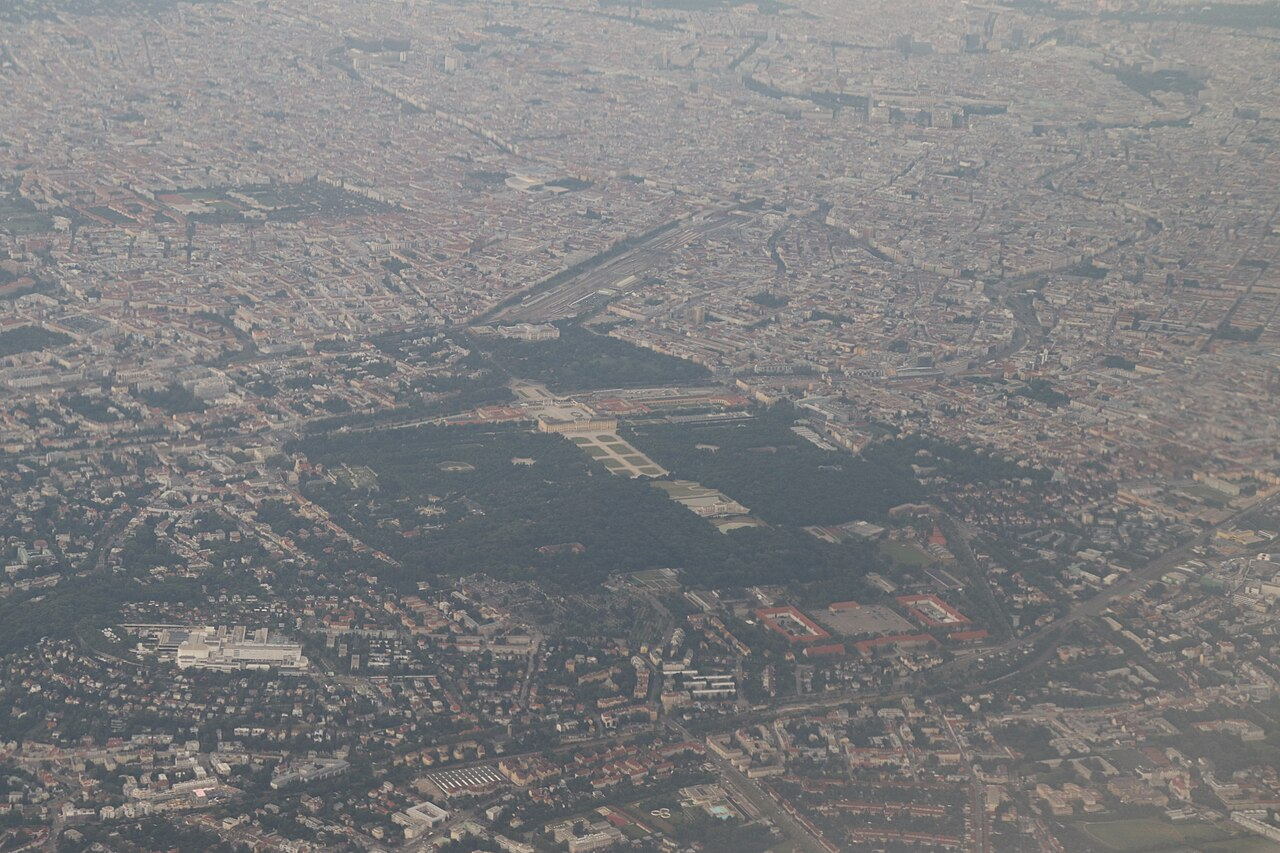
\includegraphics[width=0.88\textwidth]{images/oblique_aerial_imagery_example.jpg}
            \caption{Example of an oblique aerial view of Vienna, where perspective and building sides are visible.}
        \end{figure}
        \noindent\small Image source and licence information: \seeherefooter{https://commons.wikimedia.org/w/index.php?oldid=1107762177}.\normalsize
        
%        \bibliographystyle{plainnat}
%        \bibliography{/home/donkarlo/Dropbox/repo/nd_shared_research/bibliography/bibliography.bib}
\end{document}
